\documentclass[paper=a4, fontsize=11pt,twoside]{scrartcl}	% KOMA
\usepackage[a4paper,pdftex]{geometry}	% A4paper margins
\setlength{\oddsidemargin}{5mm}			% Remove 'twosided' indentation
\setlength{\evensidemargin}{5mm}
\usepackage[protrusion=true,expansion=true]{microtype}	
\usepackage{amsmath,amsfonts,amsthm,amssymb}
\usepackage{graphicx}
\usepackage[spanish]{babel}
\usepackage[hidelinks]{hyperref}
\usepackage{graphicx}
\usepackage{xcolor}
\usepackage{fancyhdr}
\usepackage{hyperref}
\usepackage[T1]{fontenc}
\usepackage{lmodern}
\newcommand{\HRule}[1]{\rule{\linewidth}{#1}} 	% Horizontal rule
\usepackage{float}

\graphicspath{ {./images/} }
\makeatletter							
\def\printtitle{%						
{\centering \@title\par}}
\makeatother									
\makeatletter							
\def\printauthor{%					
{\centering \large \@author}}				
\makeatother							
\title{	\normalsize \textsc{DOCUMENTO TÉCNICO} 	
		 	\\[2.0cm]								
             \HRule{0.5pt} \\						
             \LARGE \textbf{\uppercase{Sistemas de posicionamiento de objetos mediante la tecnología Bluetooth Low Energy, modo Beacon}}	
			\HRule{2pt} \\ [0.5cm]		
			\normalsize \today			
		}
\author{
    Rubén Arce Domingo\\	
		Máster en automatización y robótica\\	
        industrial\\
        akimbo170@gmail.com\\
}
\begin{document}
\thispagestyle{empty}		
\printtitle					
  	\vfill
\printauthor				
\newpage
\cleardoublepage
\tableofcontents
\listoffigures
\cleardoublepage
\pagestyle{fancy}
\fancyfoot[R]{Rubén Arce}
\fancyfoot[L]{BLE Tracking - 2021}
\section{Memoria descriptiva}
    \subsection{Antecedentes y objeto del proyecto}
        Este proyecto surge como respuesta a la necesidad de poder localizar un número elevado de equipos en 
        constante movimiento con exactitud en un espacio cerrado.
        \paragraph{}
       Los objetivos principales son los siguientes:
        \begin{enumerate}
            \item Estudiar las distintas alternativas para llevar a cabo el tracking de objetos de una forma
            sencilla y sin requerir de una gran inversión.
            \item Analizar las tecnologías existentes para la monitorización en interiores.
            \item Estudiar del parámetro Rssi como medida de la potencia de una señal y cálculo de la distancia entre equipos.
            \item Desarrollar un sistema de visualización a través de un mapa sobre el que situar los equipos en movimiento.
            \item Diseñar un hardware específico para la aplicación requerida.
            \item Programar tanto el equipo emisor como el receptor, así como del algoritmo de visualización.
            \item Comprobar el rendimiento del equipo y llevar a cabo pruebas de campo. 
        \end{enumerate}
        \paragraph{}
        Una vez fijado el alcance del proyecto se puede empezar a planificar el mismo y buscar la mejor solución 
        posible, por ello surgen los siguientes objetivos derivados de los primeros para poder sacar el producto 
        al mercado:
        \begin{enumerate}
            \item Fijar un precio muy competitivo.
            \item Desarrollar un producto estándar y de fácil aplicación.
            \item Facilitar una instalación sencilla por un usuario no técnico.
            \item Conseguir un mantenimiento escaso o nulo.
            \item Producto seguro y que esté preparado para superar los marcados UL
            (Underwriters Laboratories) y CE (Conformidad Europea) así como protecciones frente a electricidad estática.
        \end{enumerate}
    \subsection{Ámbito de aplicación}
        El tracking de objetos en espacios cerrados está incrementando su popularidad debido a que es una 
        arma de publicidad muy poderosa que demandan los grandes centros comerciales para llevar a cabo estudios de marketing
        y poder analizar el comportamiento de sus clientes.
        \paragraph{}
        El mayor nicho de mercado es aplicado a no tener que interactuar tocando los objetos, 
        esto, teniendo en cuenta los tiempos que corren, es una necesidad de numerosas empresas privadas, ayuntamientos 
        y empresas estatales.
        \paragraph{}
        A modo de resumen se engloban los principales ámbitos de aplicación de esta tecnología:
        \begin{enumerate}
            \item Marketing: Estudios de mercado y de necesidad de los clientes. Elaboración de un "heat map", o mapa 
            de las zonas con más afluencia de gente.
            \item Sanidad: Monitorización de pacientes en planta. 
            \item Seguridad: Únicamente los empleados con autorización y proximidad podrán llevar a cabo acciones,
            esto tiene sentido a la hora de no tener que dar a cada trabajador una llave que pueda replicarse.
            \item Vandalismo: Conociendo la localización de los equipos dentro de un local cerrado, en el momento 
            en el que se deja de situar un elemento en el mapa, se puede dar la voz de alarma ante un robo.
            \item Propaganda y nueva forma de publicidad: Activar acciones en función de la localización en determinados
            puntos de interés permite llevar a otro nivel las ideas de los publicistas.
        \end{enumerate}
        Vemos por tanto que hay numerosas aplicaciones y una alta demanda de este producto tecnológico, es por ello por lo que se 
        procede a explorar cual es la forma más adecuada para llevarlo a cabo e implementarlo.
    \subsection{Análisis de soluciones al tracking de objetos}
        Se plantean dos problemáticas, en primer lugar se busca llevar a cabo el seguimiento de elementos en movimiento, y por otro lado, 
        se ha de enviar esta información de alguna forma al sistema correspondiente para que lleve a cabo el análisis de los datos. Esta
        última acción es esencial en el proceso, es lo realmente interesante desde el punto de vista del cliente final de esta tecnología.
        En lo que respecta a la obtención de datos de posición relativa de objetos o personas se presentan las siguientes opciones:
        \subsubsection {Wifi}
            Llevar a cabo el tracking mediante la escucha de wifis es una posibilidad, para ello sería
            necesario que, inicialmente, se colocara un móvil en cada uno de los objetos a identificar. Esto es aceptable 
            en el caso de monitorización de personas pero inasumible para objetos.
            \paragraph{}
            El procedimiento consistiría en llevar a cabo un barrido de direcciones MACs que generan los móviles cuando tienen el wifi activado,
            es decir que este sistema no funcionaría en el caso de que una persona lleve puestos los datos del móvil únicamente.
            \paragraph{}
            Otra desventaja es el hecho de que al tener un equipo buscando wifis la información personal del propietario, es decir, localización,
            fecha, hora a la que se intentó conectar y dirección MAC que identifica y relaciona un móvil a una persona, queda expuesta.
            Se ha de tener en cuenta la política de privacidad vigente, la cual se incumpliría al emplear esta tecnología para llevar a cabo el tracking. 
            \begin{center}
                \begin{figure}[ht]
                    \centering
                    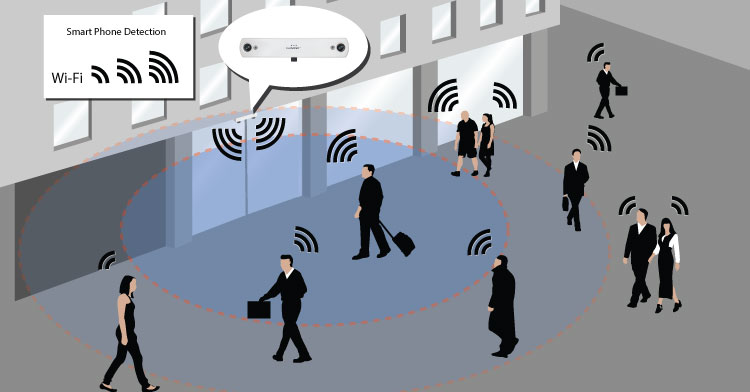
\includegraphics[width=0.4\textwidth]{WifiCounting.jpg}
                    \caption{Detección de personas aplicando redes wifi.}
                    \label{fig:mesh1}
                \end{figure}
            \end{center}
            La única solución al problema es que se ha de pedir permiso formal a la persona para poder llevar a cabo
            el tratamiento de sus datos, cosa que es dificil puesto que se desconoce quien va a llevar a cabo el uso del equipo.
            \paragraph{}
            El artículo 29 de privacidad de datos de la comunidad europea dice lo siguiente:
            “WiFi-tracking, depending on the circumstances and purposes of the data collection, such tracking under the GDPR is likely
            either to be subject to consent, or may only be performed if the personal data collected is anonymised”.
            Es por ello por lo que se tendrá en cuenta como opción aunque haya numerosos puntos en contra para implementar un sistema como este.
        \subsubsection {GPS}
            La tecnología por excelencia para llevar a cabo el seguimiento de objetos o personas es el GPS. La principal desventaja
            que presenta es el elevado consumo energético comparado con el wifi o el bluetooth.
            \paragraph{}
            Mantener un módulo GPS encendido y pretender llegar a una autonomía de años es a día de hoy
            imposible, es por ello por lo que existen dos opciones.
            O se emplea un teléfono móvil para llevarlo a cabo, cosa inviable si se intentan monitorizar objetos y no personas en
            movimiento, o el tiempo de refresco de los datos ha de ser muy lento, del orden de horas,
            cosa de nuevo inasumible para la aplicación que se presenta.
            \paragraph{}
            Por otro lado, se ha de tener en cuenta también el aumento de precio que supondría un módulo GPS sumado a la antena que lleva consigo de 
            dimensiones nada despreciables. 
            Consecuentemente, esta tecnología se tendrá en cuenta pero no es la más adecuada para la problemática presente.
        \subsubsection {Bluetooth Low Energy - Beacon}
            La tecnología Bluetooth es un estándar industrial aplicado a conexiones inalámbricas que permite transferir 
            grandes cantidades de información en distancias cortas a bajas velocidades. Puede ser enfocado a conexión
            punto a punto, o como es nuestro caso llevar a cabo una red de equipos que emiten en modo broadcast.
            \paragraph{}
            La potencia de emisión va desde los -20 dBm (0.01 mW) hasta los +20 dBm (100 mW). Cuanta mayor potencia de emisión, mayor consumo energético
            del dispositivo, pero también conseguiremos una mayor distancia de escaneo.
            \paragraph{}
            La forma de envío de datos que más encaja dentro de la tecnología BLE (Bluetooth Low Energy) es Beacon o baliza, un 
            dispositivo que transmite una señal de bluetooth cada cierto tiempo y es visible por cualquier otro equipo que escuche 
            en esa misma frecuencia. La principal ventaja es que no es necesario llevar a cabo la conexión al equipo que escucha.
            Existen varios tipos de beacons:
            \begin{enumerate}
                \item iBeacon: Fue la primera tecnología BLE Beacon desarrollada por Apple. Permite leer y emitir en modo 
                broadcast para cualquier dispositivo que disponga de Bluetooth low energy. Es un protocolo propietario, es 
                decir es un estándar cerrado. 
                Los iBeacons disponen de los siguientes identificadores:
                \begin{itemize}
                    \item UUID: Indentificador único del dispositivo, una cadena de carácteres de 16 bytes
                    que permite caracterizar a cada equipo.
                    \item Major: Número entero de 0 a 65535, se usa para identificar grupos, un ejemplo sería 
                    asignar un Major común para todos los beacons de una misma planta o habitación.
                    \item Minor: Es también un número entero de 0 a 65535 que se emplea para distinguir un Beacon
                    específico dentro de un grupo, entendiéndose como grupo aquellos beacons con mismo valor de Major.
                \end{itemize}
                \begin{center}
                    \begin{figure}[ht]
                        \centering
                        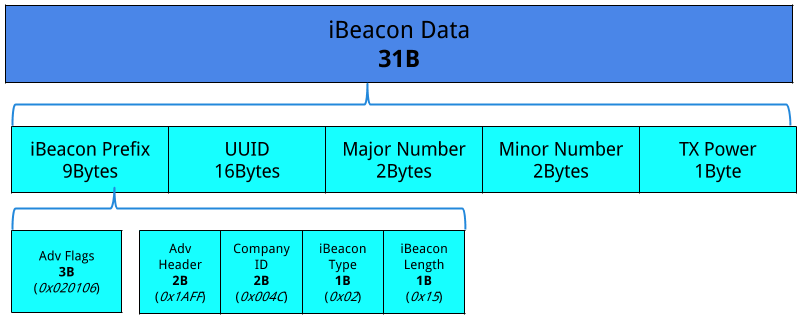
\includegraphics[width=0.6\textwidth]{tipos_beacon_ibeacon.PNG}
                        \caption{Trama de bytes de cabecera de modo iBeacon (Apple).}
                        \label{fig:mesh2}
                    \end{figure}
                \end{center}
                \item Eddystone: Creado por Google, es un protocolo de código abierto. A diferencia del protocolo anterior este 
                permite transmitir:
                \begin{itemize}
                    \item URL: Un url propio de una web, de esta forma se evita la necesidad de tener que contar con una app instalada.
                    \item UID: Similar al UUID del iBeacon, este parámetro identifica al Beacon y permite llevar acciones individuales.
                    \item TML: Permite enviar información relativa al Beacon, como por ejemplo, el porcentaje de batería o valores de sensores.
                \end{itemize}
                \begin{center}
                    \begin{figure}[ht]
                        \centering
                        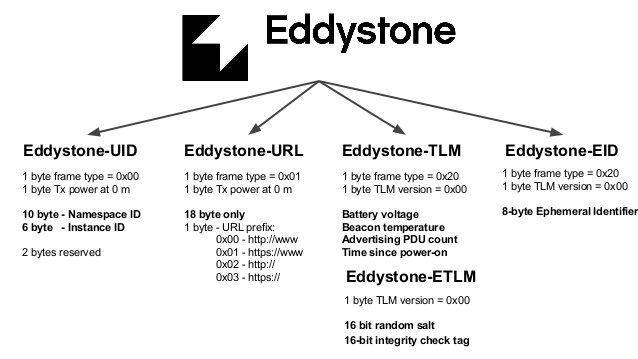
\includegraphics[width=0.5\textwidth]{tipos_beacon_edison.PNG}
                        \caption{Modo Beacon Edison (Google) }
                        \label{fig:mesh3}
                    \end{figure}
                \end{center}
                \item AltBeacon: Es un protocolo de código abierto que surge como resultado de las incompatibilidades de las dos 
                tecnologías anteriores, la ventaja principal es que permite más flexibilidad de modificaciones así como compatibilidad 
                entre sistemas operativos.
    \subsection{Análisis de opciones de subida de datos}
        Una vez exploradas las opciones de posicionamiento de los equipos se llevará a cabo el estudio de posibilidades de subida de estos datos
        a la nube, es por ello por lo que se contemplarán varias opciones:
        \subsubsection {MQTT}
            MQTT (Message Queing Telemetry Transport) es un protocolo estándar aplicado principalmente al IoT (Internet of Things). Está basado en publicación y 
            suscripción con un servicio de mensajería push. Los mensajes se publican en topics, sobre los cuales los distintos 
            dispositivos se encuentran escuchando.
            La base de la comunicación es el Broker, encargado de dar soporte a todos los topics, los clientes inician una 
            conexión TCP/IP con él que se mantiene abierta constantemente hasta que el cliente la finalice. Se emplean los puertos
            1883 o 8883 con seguridad TLS.
            Cada mensaje tiene un QoS (Quality of service), es el mecanismo de calidad del servicio, o lo que es lo mismo es la forma de
            gestionar la robustez de los mensajes entre clientes y ante los fallos de conectividad.
            \begin{itemize}
                \item QoS 0: Envío una única vez
                \item QoS 1: Mensaje enviado hasta que se garantiza que se entrega.
                \item QoS 2: Garantizado que cada mensaje se entrega al suscriptor por una única vez.
            \end{itemize}
            Esta es una opción para conseguir que los equipos que escuchan a los beacons envíen a un mismo
            topic la información obtenida por bluetooth. Será el sistema de visualiación el que esté escuchando también en 
            el mismo topic.
        \subsubsection {HTTP Post}
            A través del protocolo de transferencia de hipertexto se puede llevar a cabo una petición post, la cual consiste en que
            un servidor acepte los datos recibidos por el microcontrolador.
            La ventaja es que con el HTTP post solo se mantiene la conexión abierta al hacer la conexión, luego se desconecta hasta 
            la siguiente vez en la que se vuelvan a publicar datos. 
            \paragraph{}
            Otra ventaja es que mediante peticiones se pueden transferir datos a distintos servidores.
            Por el contrario, con MQTT solo se puede enviar información a aquellos servidores que estén suscritos al mismo tópic que el dispositivo.
            \paragraph{}
            El principal inconveniente es que está demostrado que en una red 3G, una petición post es del orden de 93 veces
            más lenta que un mensaje MQTT, con el consiguiente consumo energético que esto conlleva. Otro inconveniente es el hecho 
            de que se requiera de un servidor con una API o endpoint que esté constantemente escuchando a los distintos posts.
        \subsubsection {ESP Now}
            Se plantea la opción de que no todos los equipos que escuchan a los beacons dispongan de conexión a internet, es por ello
            por lo que se baraja la posibilidad de llevar a cabo una red de elementos que escuchan y que envían a un único concentrador encargado de enviar
            esta información a internet por cualquier otro método.
            Es decir, se contempla la opción de establecer una red de elementos que escuchan, para lo cual se emplea 
            un protocolo de comunicación rápido denominado ESP-NOW, que tiene las siguientes características:
            \begin{itemize}
                \item Encriptación de las comunicaciones.
                \item Hasta 250 Bytes de payload o mensaje a enviar.
                \item Rapidez de comunicación entre microcontroladores.
            \end{itemize}
            \paragraph{}
            La idea sería la siguiente:
            \begin{enumerate}
                \item El equipo que lleva a cabo el barrido y búsqueda de beacons escanea e intenta conectarse a 
                internet por wifi.
                \item Si lo consigue publica los datos, en el caso de que falle enviará por ESP NOW la información
                que no puede subir a internet a otro equipo en su misma red que si que pueda.
                \item Este segundo hará lo mismo hasta que finalmente alcance con uno que sí que pueda subir estos datos.
            \end{enumerate}
            \begin{center}
                \begin{figure}[ht]
                    \centering
                    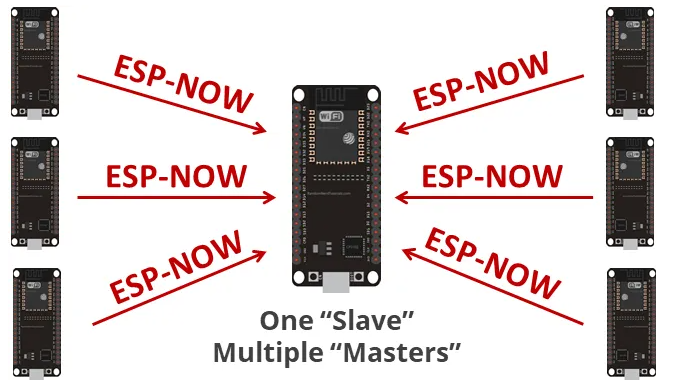
\includegraphics[width=0.4\textwidth]{espnow.PNG}
                    \caption{Diagrama explicativo de una red de ESP32.}
                    \label{fig:mesh4}
                \end{figure}
            \end{center}
        \end{enumerate}
    \subsection{Resultados finales}
        Una vez analizadas las dos problemáticas y las distintas soluciones a cada una de ellas, se ha confeccionado la siguiente tabla 
        en la que se puede ver una comparativa entre cada una de ellas.

        Por un lado está la forma en la que poder medir las distancias de los equipos con respecto a los equipos que escuchan,
        se contemplan las siguientes opciones:
        \begin{center}
            \addcontentsline{lot}{table}{Comparativa de opciones de posicionamiento}
            \begin{tabular}{|c | c| c| c| c |} 
            \hline
            Tecnología  & Coste  & Complejidad & Distancia & Consumo energético \\ [0.5ex] 
            \hline
            GPS& Elevado& Baja & Ilimitada& Muy alto\\
            Wifi& Medio& Media & ~ 100 m & Alto\\ 
            Bluetooth& Bajo& Media & ~ 100 m & Muy bajo\\ 
            \hline
            \end{tabular}
        \end{center}   
        El claro ganador en este caso es el Bluetooth, debido, principalmente, al precio que supondría llevar a cabo una red de estas 
        características, así como el bajo consumo energético que hace que el mantenimiento de los equipos sea casi inexistente.
        \paragraph{}
        Recordemos que una de las premisas iniciales era que los equipos requieran poco cuidado por parte del cliente, 
        lo que se consigue empleando esta tecnología en la que solo es necesario cambiar una pila una vez al año.
        \paragraph{}
        En lo que respecta a la comunicación de estos datos de distancia entre equipos a internet, se ha reunido de nuevo en la 
        siguiente tabla un resumen con las opciones y los puntos a favor y en contra de cada una de las tecnologías.
        \begin{center}
            \addcontentsline{lot}{table}{Comparativa de opciones de subida de datos a Internet}
            \begin{tabular}{||c | c| c| c||} 
            \hline
            Tecnología  & Velocidad de datos & Coste & Complejidad \\ [0.5ex] 
            \hline
            MQTT& Elevada  & No & Baja\\
            HTTP POST& Baja & Medio & Baja\\ 
            ESP NOW& Media & No & Alta\\ 
            \hline
            \end{tabular}
        \end{center}   
        La elección en este caso está mucho más ajustada, en el caso de que se pueda conectar a todos los equipos que 
        escuchan a internet el ganador será la opción de MQTT, puesto que es la forma más fácil de llevar a cabo el envío de datos.

        Si que no llegara la señal wifi a todos los puntos en los que se decida llevar a cabo el tracking de objetos 
        surge un problema puesto que perderemos esos datos. La solución es hacer que este equipo, que no tiene conexión a internet,
        envíe los datos por ESP NOW a otro que si que sea capaz de subir tanto su información como la de su compañero al broker por MQTT.

        Puesto que se pretende llevar a cabo un sistema válido para toda la casuística de instalaciones, se han contemplado ambas opciones
        y la implementación real llevará a cabo los dos métodos.
        
        Es decir, que la única opción desechada ha sido la conexión directa con un servidor mediante HTTP debido a que, en primer
        lugar sería necesario programar un servicio que escuchará en este endpoint y luego sería necesario hostearlo 
        para que disponga de una IP pública estática y sea accesible desde cualquier parte del mundo.
    \subsection{Planificación}
        \paragraph{}
        Para sintetizar el proceso de desarrollo del proyecto técnico se empleará un diagrama GANTT. En la
        figura 5 podemos ver la evolución del desarrollo del mismo así como la duración exacta de cada etapa. 
        \begin{center}
            \begin{figure}[H]
                \centering
                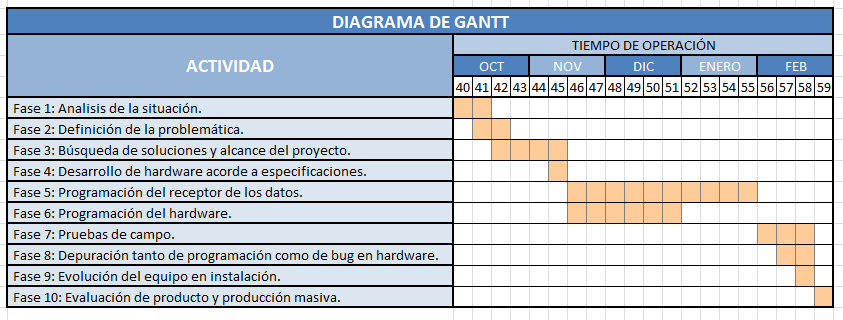
\includegraphics[width=1\textwidth]{diagrama de gantt.PNG}
                \caption{Diagrama de GANTT del proyecto.}
                \label{fig:mesh18}
            \end{figure}
        \end{center} 
\section{Memoria justificativa}
    \subsection{Cálculos justificativos de la instalación}
        En este apartado se llevará a cabo el estudio de la viabilidad del proyecto desde el punto de vista
        técnico, para lo cual se contemplará un estudio del Rssi como forma de medir distancia, un análisis 
        de la previsión energética de los equipos, un análisis del las frecuencias y ganancias de las antenas 
        empleadas.
    \subsection{Cálculo de distancia por Rssi}
        \subsubsection{Rssi}
            \paragraph{}
            El Rssi (Received signal strength indicator) es un indicador de la energía o potencia recibida en un mensaje de radio. 
            Está asociado con la atenuación de la señal, cuanto más pequeña es su valor menor atenuación. Este valor está 
            presente no solo en Bluetooth sino también en el Wifi (2,4 GHz) o en las bandas de radio industriales, científicas y médicas,
            las denominadas ISM (desde 433MHz a 458.5MHz y desde 860MHz a 960MHz)
            \paragraph{}
            De las muestras obtenidas en pruebas de campo con bluetooth se puede concluir que es posible llegar a estimar la distancia
            a partir de los valores de Rssi con un error que disminuye cuanto más alejados se encuentren los elementos a medir. 
            \paragraph{}
            Los rangos del Rssi se obtienen bien por aproximaciones teóricas o bien por experimentación. Esto es debido a que 
            es fuertemente alterado por las condiciones del medio en el que se encuentre. Asimismo es importante mencionar que
            este parámetro es medido a través de un hardware que rara vez tiene un comportamiento idéntico, eso explica las fluctuaciones 
            también.
            \paragraph{}
            Los modelos de cálculo del Rssi se basan en la pérdida de señal en el espacio, como sabemos la potencia de la señal
            disminuye con el cuadrado de la distancia. Esta ecuación de Friis para la transmisión libre en el espacio es 
            una fórmula teórica, existen aproximaciones obtenidas por métodos empíricos:
            \begin{equation}
                P_L(d) [dB] = P_L(d_0) [dB] + 10n * \log_{10} \frac{d_i}{d_0} 
            \end{equation}
            \paragraph{}
            Siendo PL (d0) la pérdida de propagación a 1 metro y n una constante que depende del medio, será igual
            a 2 si se encuentra en el espacio libre sin obstáculos ni reflexiones o dispersiones de señal.
            \paragraph{}
            Para calcular este parámetro n se ha de aplicar la siguiente fórmula, como podemos ver para llevar a cabo el 
            cálculo se han de tomar valores empíricos de potencias:
            \begin{equation}
                n = \frac{ P_L(d_i) - P_L(d_0) }{10n*\log_{}\frac{d_i}{d_0}}
            \end{equation}
            \paragraph{}
            Por lo tanto, y una vez obtenidos los valores de potencia a distintas distancias, podemos obtener la ganancia
            de la señal recibida:
            \begin{equation}
                Rssi [dBm] = -10n*\log_{10} d+ A[dBm]
            \end{equation}
            \paragraph{}
            Disponiendo ya del valor de la constante de pérdidas, d, calculado con la ecuación (2) y los valores
            de Rssi medidos desde la antena receptora a 1 metro de distancia, (3), podemos obtener:
            \begin{equation}
                d= 10^\frac{-(Rssi - A)}{10n}
            \end{equation}
            Llevados a cabo los cálculos por parte del equipo que escucha a los distintos beacons, podemos calcular la distancia 
            real a cada uno de ellos. En el caso de que se solapen y dos receptores escuchen el mismo Beacon será necesario
            llevar a cabo el proceso de trilateración expuesto a continuación.
            Para comprobar la fluctuación del parámetro del Rssi se ha llevado a cabo la toma de este parámetro a lo largo de un 
            periodo de tiempo largo y los resultados a 2 metros y a 3 metros se encuentran respectivamente en la figura 6. 
 
            Podemos ver que hay pequeñas flucuaciones y es por ello por lo que será necesario implementar un sencillo filtro para
            evitar el ruido electromagnético que hemos visto anteriormente.
            
            Se ha llevado a cabo la prueba de incrementar el número de iBeacons y situarlos a la misma distancia del 
            equipo que escucha, los resultados se muestran en la figura 7.
            
            Análogamente las diferencias son notables, esto demuestra la necesidad de implementar
            un filtro que no falsee las medidas y cree distancias incoherentes puntuales entre los equipos.
            
            El filtro más habitual para este tipo de aplicaciones es el denominado Kalman Filter:
            \begin{equation}
                Rssi_{suavizado} = \alpha * Rssi_{n} + (1-\alpha) * Rssi_{(n-1)}
            \end{equation}
            Otra opción que experimentalmente ha dado buenos resultados es la de selecionar los 20 valores anteriores,
            obtener la media y si se separa más de un 40\% el valor nuevo lo rechazo. Con esto consigo eliminar las 
            fluctuaciones indesadas que se podían apreciar en la figura 6.
            \begin{center}
                \begin{figure}[ht]
                    \centering
                    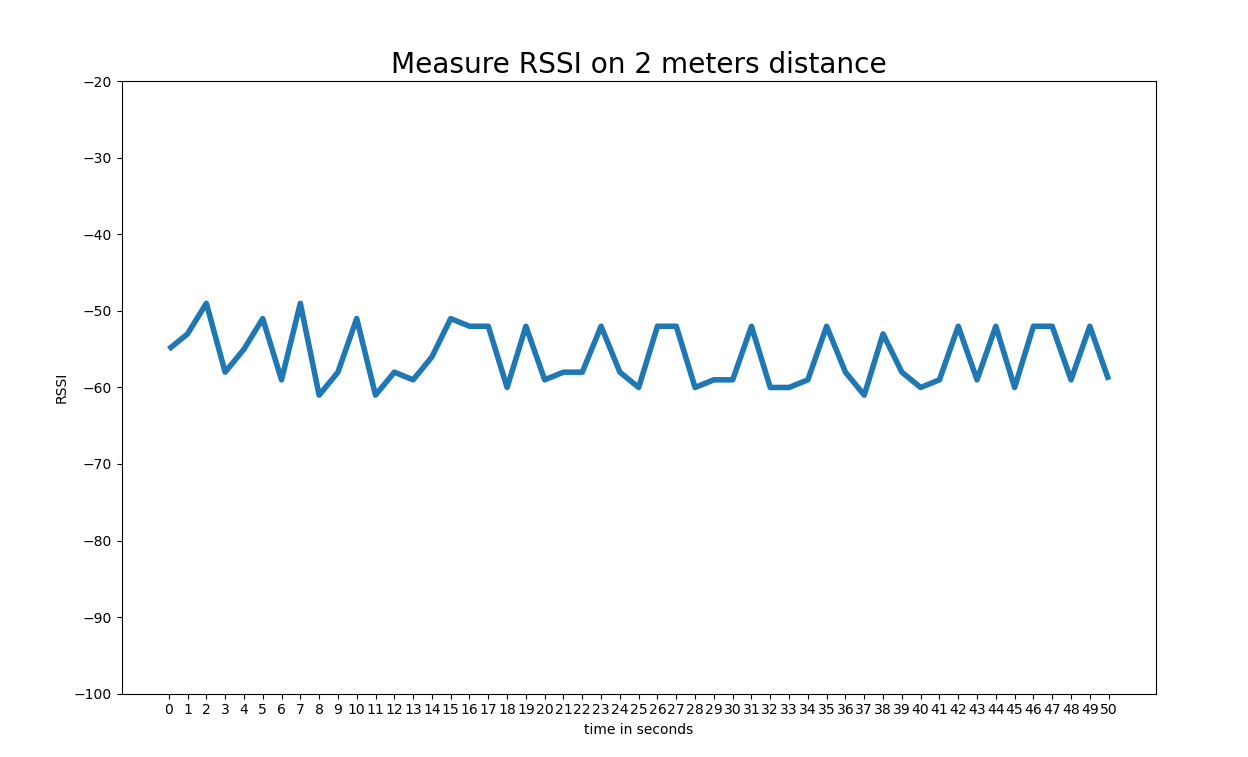
\includegraphics[width=0.6\textwidth]{1_beacon_2_meters.PNG}
                    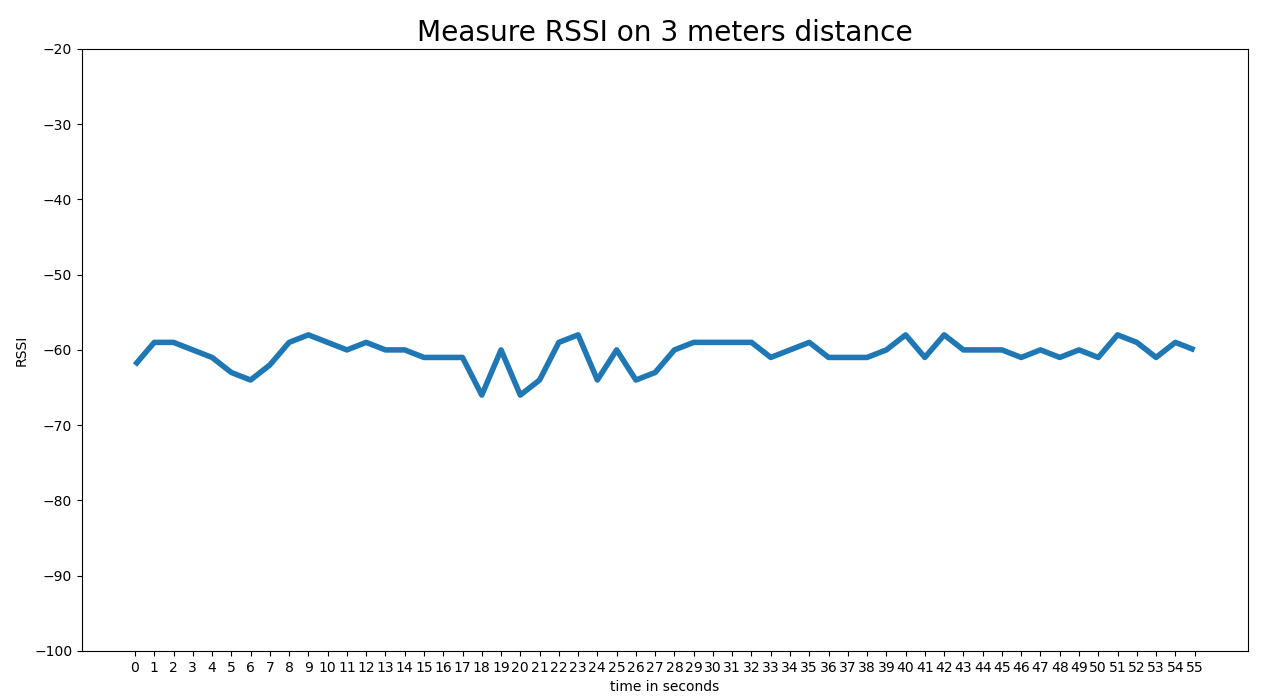
\includegraphics[width=0.55\textwidth]{1_beacon_3_meters.PNG}
                    \caption{Prueba de campo, medición Rssi de Beacons a 2 y 3 metros.}
                    \label{fig:mesh5}
                \end{figure}
            \end{center}
            \begin{center}
                \begin{figure}[ht]
                    \centering
                    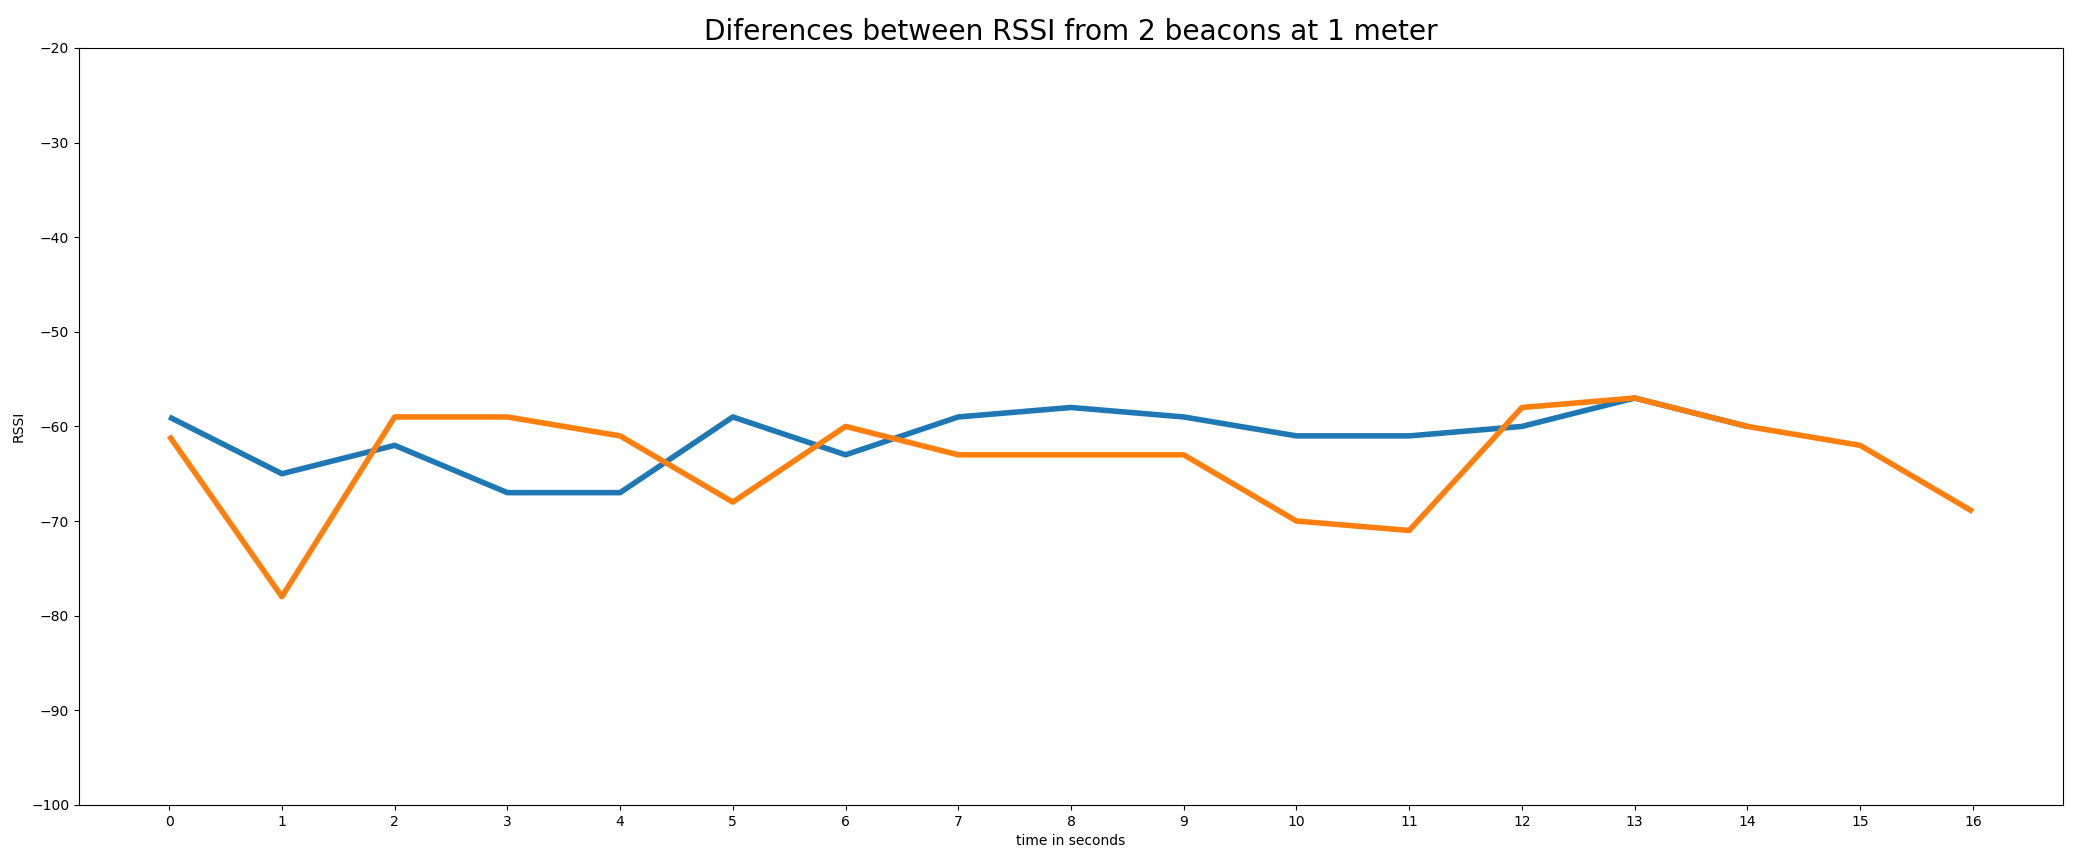
\includegraphics[width=0.6\textwidth]{10min_2beacons_same_distance.PNG}
                    \caption{Variaciones de Rssi entre beacons a distancias iguales.}
                    \label{fig:mesh6}
                \end{figure}
            \end{center}

        \subsubsection{Trilateración y posicionamiento}
            Una vez obtenidas las distancias a los distintos equipos de receptores es necesario llevar a cabo el
            posicionamiento exacto de los mismos, para ello se emplea la trilateración:
            \begin{center}
                \begin{figure}[H]
                    \centering
                    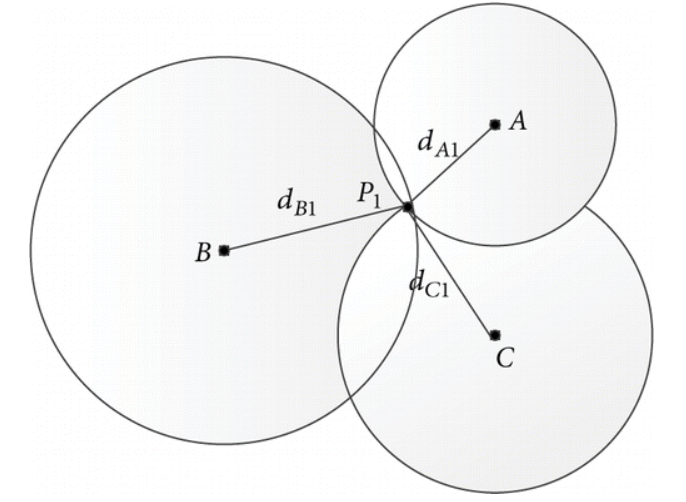
\includegraphics[width=0.4\textwidth]{trilateration_circle.png}
                    \caption{Trilataración con tres equipos escuchando al mismo Beacon.}
                    \label{fig:mesh7}
                \end{figure}
            \end{center}
                Hemos de resolver las siguientes ecuaciones básicas sobre la distancia entre recta y un punto en 
                una circunferencia, en la figura 8 podemos verlo gráficamente.
                \begin{equation}
                    d_{A1}= \sqrt[]{(x-x_A)^2+(y-y_A)^2}
                \end{equation}
                \begin{equation}
                d_{B1}= \sqrt[]{(x-x_B)^2+(y-y_B)^2}
                \end{equation}
                \begin{equation}
                    d_{C1}= \sqrt[]{(x-x_C)^2+(y-y_C)^2}
                \end{equation}
                Llevando a cabo la simplificación obtenemos un sistema de ecuaciones que permite calcular la distancia
                relativa a cada uno de los equipos que escuchan. En el anexo de software se muestran los resultados con mayor 
                detalle. En la figura 9 podemos ver un adelanto del posicionamiento de carros de la compra en un supermercado.
                \begin{center}
                    \begin{figure}[h]
                        \centering
                        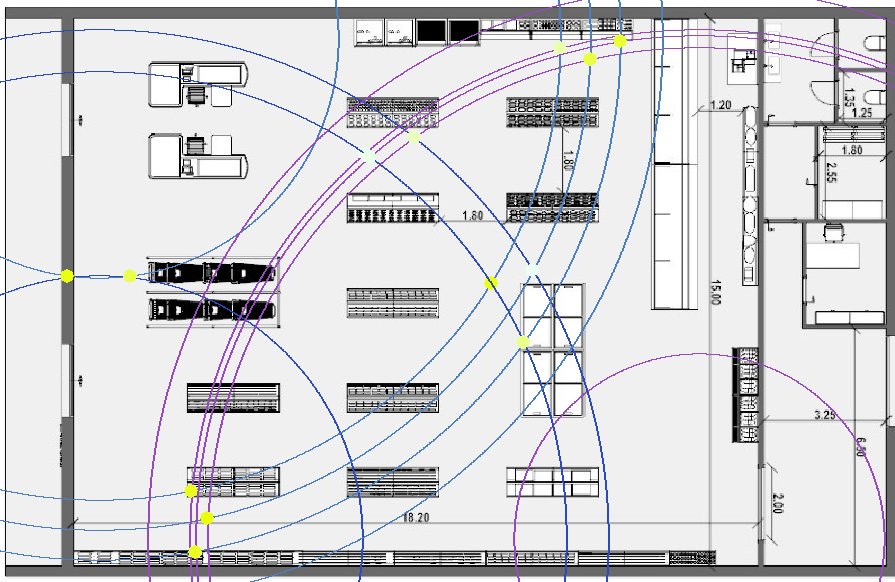
\includegraphics[width=0.7\textwidth]{agrupation_3.PNG}
                        \caption{Posicionamiento de los beacons en carros de supermercado.}
                        \label{fig:mesh7}
                    \end{figure}
                \end{center}
                \paragraph{}
                % \url{https://journals.sagepub.com/doi/full/10.1155/2014/371350#:~:text=Rssi%3DPt%2DPL(d).&text=In%20this%20formula%2C%20Pt,%2DPL(d).}
    \subsection{Cálculo de consumos energéticos}
            El procesador empleado, tanto para el equipo emisor como para el receptor, disponen de los siguientes modos de funcionamiento:
            \begin{itemize}
                \item  Active Mode: 160-260mA. Los dos cores del procesador encendidos, así como el procesador ULP,
                RTC, Wifi, Bluetooth, Radio, Peripherals.
                \item  Sleep mode: 3-20mA. Activos los dos cores, el coprocesaror ULP coprocessor y el RTC, inactivos el 
                Wifi, Bluetooth, Radio y periféricos.
                \item  Light sleep mode: La CPU está pausada apagando los pulsos de su reloj interno, sin embargo, el RTC
                y el coprocesador ULP se mantienen activos. Esto supone un consumo menor que en los anteriores modos de funcionamiento,
                se puede llegar a los 0.8mA.
                \item Deep sleep mode: tanto la CPU como gran parte de la RAM, así como todos los periféricos se mantienen 
                apagados. Las únicas parte no apagadas son los RTC de los periféricos y de la CPU (incluyendo el ULP) y su
                memoria interna. El chip consume en torno a los 0.15 mA si se mantiene encendido el ULP y  10µA si no.
                En el modo deep sleep todo se encuentra apagado, por ello los datos de la memoria del rtc se pierden
                puesto que se encuentra en reinicio el uC.
                \item Hibernation mode: A diferencia del modo deep sleep el oscilador de 8MHz y el ULP se encuentran apagados,
                no es posible almacenar nada de información. Tan solo el RTC funcinando con el reloj de baja velocidad puede funcionar.
                En este modo de funcionamiento el micro consume sobre los 2.5µA.
            \end{itemize}
            \begin{center}
            \addcontentsline{lot}{table}{Consumos energéticos ESP32.}
                \begin{tabular}{||c || c ||} 
                \hline
                Modo del ESP32  & Consumo energético  \\ [0.5ex] 
                \hline
                Wi-Fi Tx a 13dBm~21dBm & 160~260mA  \\ 
                Wi-Fi/BT Tx  a packet 0dBm	 & 120mA  \\
                Wi-Fi/BT Rx and listening & 80~90mA  \\
                Sleep mode &  3-20mA   \\
                Light sleep mode &0,8mA  \\
                Deep sleep mode &   0,15 mA - 10µA  \\
                Hibernation mode & 2,5µA  \\
                \hline
                \end{tabular}
            \end{center}
            A la hora de llevar a cabo la decisión sobre cómo llevar a cabo el protocolo de comunicación se ha de tener en cuenta 
            el consumo de los equipos, en especial en lo que respecta a los beacons.
            \paragraph{}
            Es por ello por lo que se ha optado por dormir al equipo durante 58 segundos, despertarlo,
            enviar su trama bluetooth y luego dormirlo hasta la siguiente vez que despierte.
            Con esto conseguimos un consumo que varía en función de la frecuencia de envío. En las siguiente tablas
            se puede ver un análisis en función del tiempo y en consecuencia la duración media de las baterías.
            Se ha puesto como ejemplo una frecuencia de envío de 10 minutos.
            \begin{center}
                \addcontentsline{lot}{table}{Frecuencia de envío frente a consumo medio.}
                \begin{tabular}{||c || c ||} 
                \hline
                Frecuencia de envío  & Consumo energético  \\ [0.5ex] 
                \hline
                1 min &  2,415 mA \\
                5 min &  0,495 mA \\ 
                10 min &  0,255 mA \\ 
                15 min &  0,175 mA \\ 
                30 min &  0,095 mA \\ 
                \hline
                \end{tabular}
            \end{center}
            \begin{center}
                \addcontentsline{lot}{table}{Frecuencia de envío frente a consumo medio.}
                \begin{tabular}{|c | c| c| c |} 
                \hline
                    Tipo de batería & Capacidad  & Autonomía(días) & Autonomía(días)   \\ [0.5ex] 
                    & (mAh) &  f=10 min &  f=5 min   \\ [0.5ex] 
                \hline
                \hline
                    Pila CRC 2032 &  240 mAh  & 39   & 20 \\ 
                    Pila AA       &  2500 mAh & 409  & 210 \\ 
                    Batería Li-Ion&  1600 mAh & 261  & 135 \\ 
                \hline
                \end{tabular}
            \end{center}
            Podemos ver por lo tanto como con una pila AA se podría llegar a conseguir sin problemas una autonomía de casi un 
            año, es por esta razón y por el tamaño reducido por lo el que se va a optar por esta solución.
            
    \subsection{Cálculo de ganancia de antenas}
            Una antena convierte la enegía electrica del transmisor en energía electromagnética y viceversa, las antenas pueden ser 
            para recibir, para transmitir o ambas. La localización de la antena, las dimensiones y el diseño pueden afectar drásticamente
            en el funcionamiento óptimo de la red de beacons. 
            Las antenas típicas en aplicaciones de radiofrecuencia con bluetooth son de -10dBm a 10dBm.

            El denominado path loss o atenuación de la señal de radio es la reducción de la densidad de potencia de una onda durante la 
            propagación en el espacio. Este parámetro es esencial a la hora de poder establecer una red de bluetooth de estas dimensiones.
            Las dimensiones de la antena se pueden llegar a obtener mediante:
            \begin{equation}
                f(Hz)=\frac{v(m/s)}{\lambda(m)}
            \end{equation}
            \begin{equation}
                \lambda_0(m)=\frac{v_0(m/s)}{f(Hz)} = \frac{2,998*10^8}{2,4*10^9} = 12,49 cm
            \end{equation}
            Para la aplicación que tenemos existen dos tipos de antenas:
            \begin{itemize}
                \item  Antenas monopolo $\lambda$/4: Menor tamaño pero menor eficiencia. 
                \item  Antenas dipolo $\lambda$ /2: Mayor tamaño pero mejores resultados.
            \end{itemize}
            Teniendo en cuenta que esta antena estará en una caja más grande y a la vista el tamaño no será un limitante.
            A modo de ejemplo en la figura 10 se muestra como es internamente cada una de las antenas.
            \begin{center}
                \begin{figure}[h]
                    \centering
                    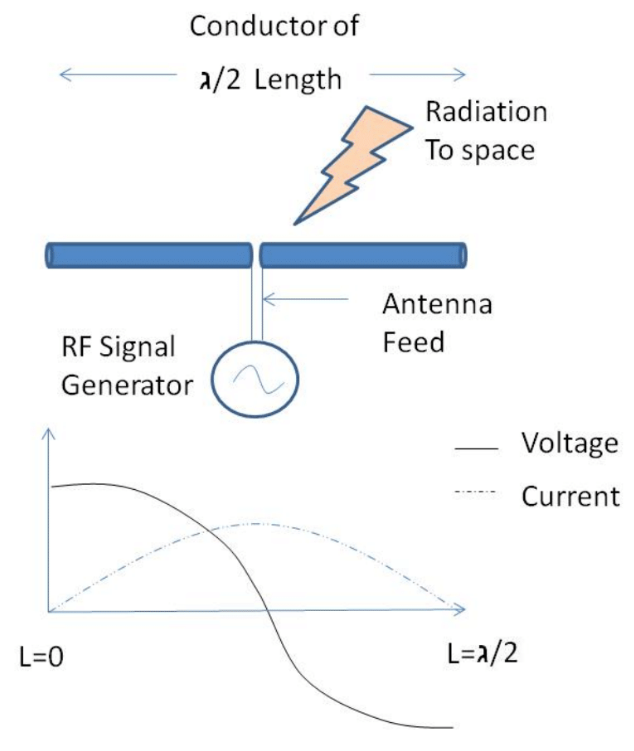
\includegraphics[width=0.4\textwidth]{antenna_design.png}
                    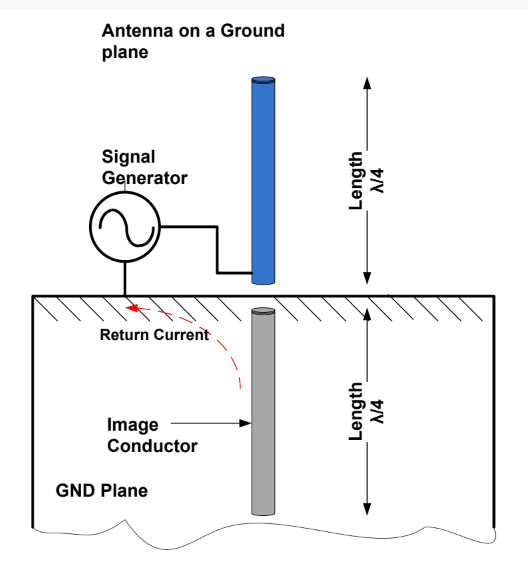
\includegraphics[width=0.45\textwidth]{antenna_design_monopole.png}
                    \caption{Diferencia entre antena de media o cuarto de $\lambda$.}
                    \label{fig:mesh8}
                \end{figure}
            \end{center}
            Además se ha de tener en cuenta que las antenas atienden a su diagrama de radiación, es decir, al
            espectro tridimensional de emisión. Según la forma de radiación podemos distinguir.
            \begin{itemize}
                \item  Antenas isotrópica: Emite con la misma densidad en todas las direcciones.
                \item  Antenas omnidireccionales: Emite en torno a un solo plano isotrópico.
                \item  Antena directiva: Concentra la energía radiada en tan solo una dirección del espacio.
            \end{itemize}
            En la figura 11 podemos ver los lóbulos de emisión y recepción de radiofrecuencia de las distintas antenas.
            \begin{center}
                \begin{figure}[h]
                    \centering
                    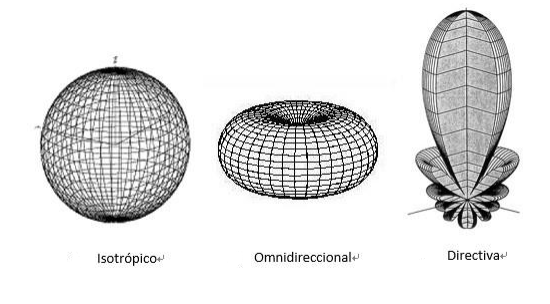
\includegraphics[width=0.8\textwidth]{antenna_types.PNG}
                    \caption{Tipos de antena en función del espectro de emisión.}
                    \label{fig:mesh10}
                \end{figure}
            \end{center}
            Dentro del mundo de las antenas existen numerosos modelos y opciones que se enumeran a continuación:
            \begin{enumerate}
                \item Antenas de cable: son las más sencillas de todas y como su propio nombre indica es un simple cable soldado a la PCB de una dimensión determinada, la cual se corresponde con la de una antena monopolo $\lambda$/4. El cable aporta el mayor rendimiento y rango de radiofrecuencia debido a sus dimensiones y a su caracter flexible, moldeable y orientable sin importar  la posición de la tarjeta.
                \item Antena PCB: es una pista en el propio circuito impreso que puede tener numerosas formas, a diferencia de la de cable esta solo se encuentra en el espacio 2D. Tiene menos eficiciencia que las anteriores y requiere más espacio pero son incluso más baratas.
                \item Antena de chip: este tipo de antena es una tarjeta o módulo que ocupa menos espacio que cualquiera de las anteriores y tiene un rendimiento intermedio entre ambas otras dos opciones.
            \end{enumerate}
            Por otro lado, se han llevado pruebas de campo con distintos modelos y distintas posiciones dentro de la caja, a continuación se muestran las 
            antenas con las que se han llevado a cabo las pruebas reales en la figura 12. 
            \begin{center}
                \begin{figure}[ht]
                    \centering
                    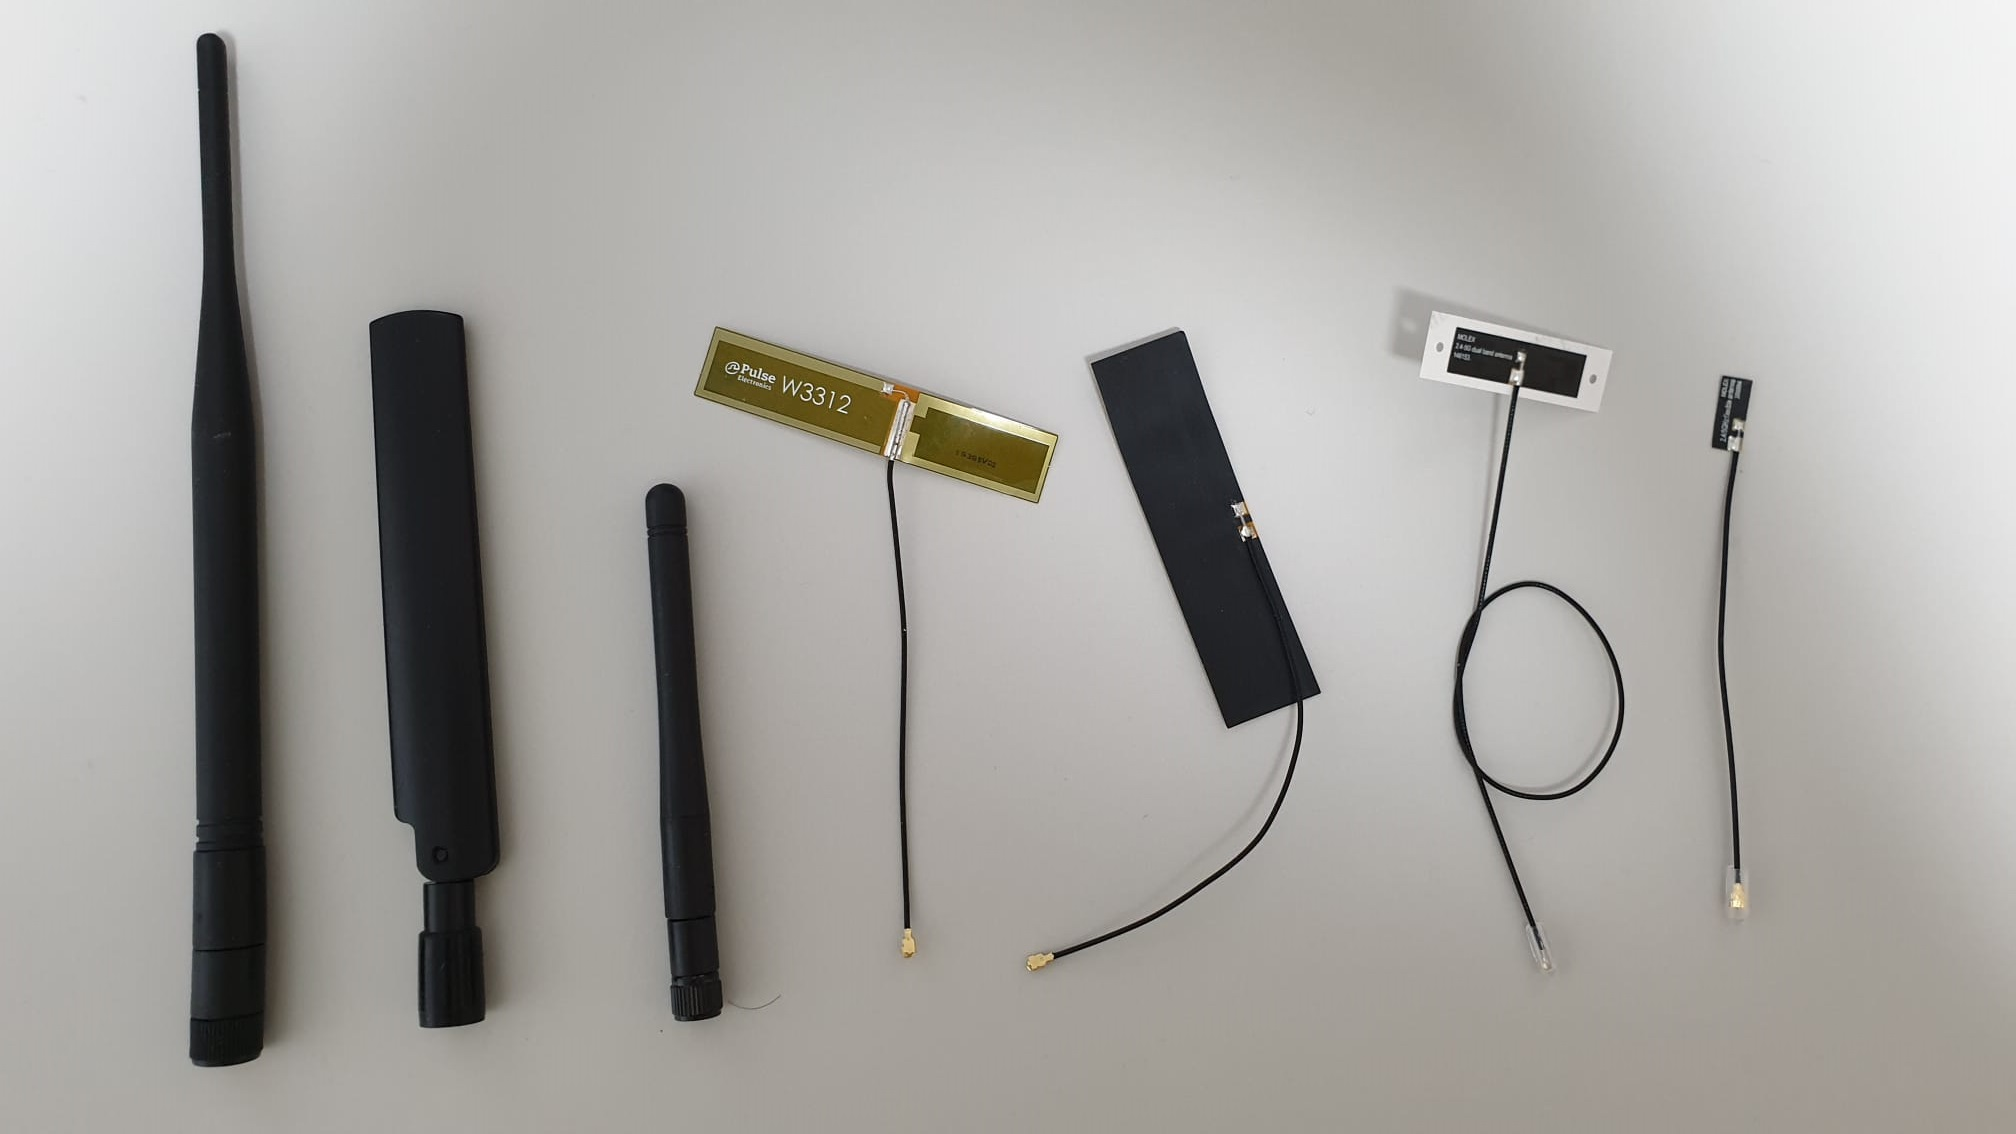
\includegraphics[width=0.5\textwidth]{antennas_variety.jpeg}
                    \caption{Tipos de antena durante las pruebas de campo.}
                    \label{fig:mesh11}
                \end{figure}
            \end{center}
            Las conclusiones obtenidas son que las antenas pcb de $\lambda$ /2 obtienen más uniformidad en las medidas a igual distancia,
            mientras que las antenas de cable ofrecen mayor rango pero son menos discretas. En definitiva, la antena es algo esencial y más 
            allá del modelo elegido prioriza más el hecho de que todos los equipos de la red dispongan de exactamente el mismo diseño.
\section{Planos}
    \subsection{Planos mecánicos}
        Los planos catalogados como mecánicos hacen referencia a la estructura de plástico
        que sostiene y protege a la electrónica de las condiciones ambientales y de contacto directo con las 
        personas.

        En el anexo de diseño mecánico se especifica con mayor detalle el procedimiento y el prototipado con impresora
        3D. A este respecto se presentan dos planos:
        \begin{itemize}
            \item Chasis de receptor o gateway
            \item Chasis de emisor o Beacon
        \end{itemize}
    \subsection{Planos eléctricos}
        Los circuitos eléctricos de la electrónica desarrollada que se presentan son los siguientes:
        \begin{itemize}
            \item Esquemático del emisor Beacon y esquemático del receptor ESP32
            \item PCB circuito del emisor Beacon y PCB circuito del receptor ESP32
        \end{itemize}
        En en el anexo de diseño eléctrico se explican con mayor detalle.
    % 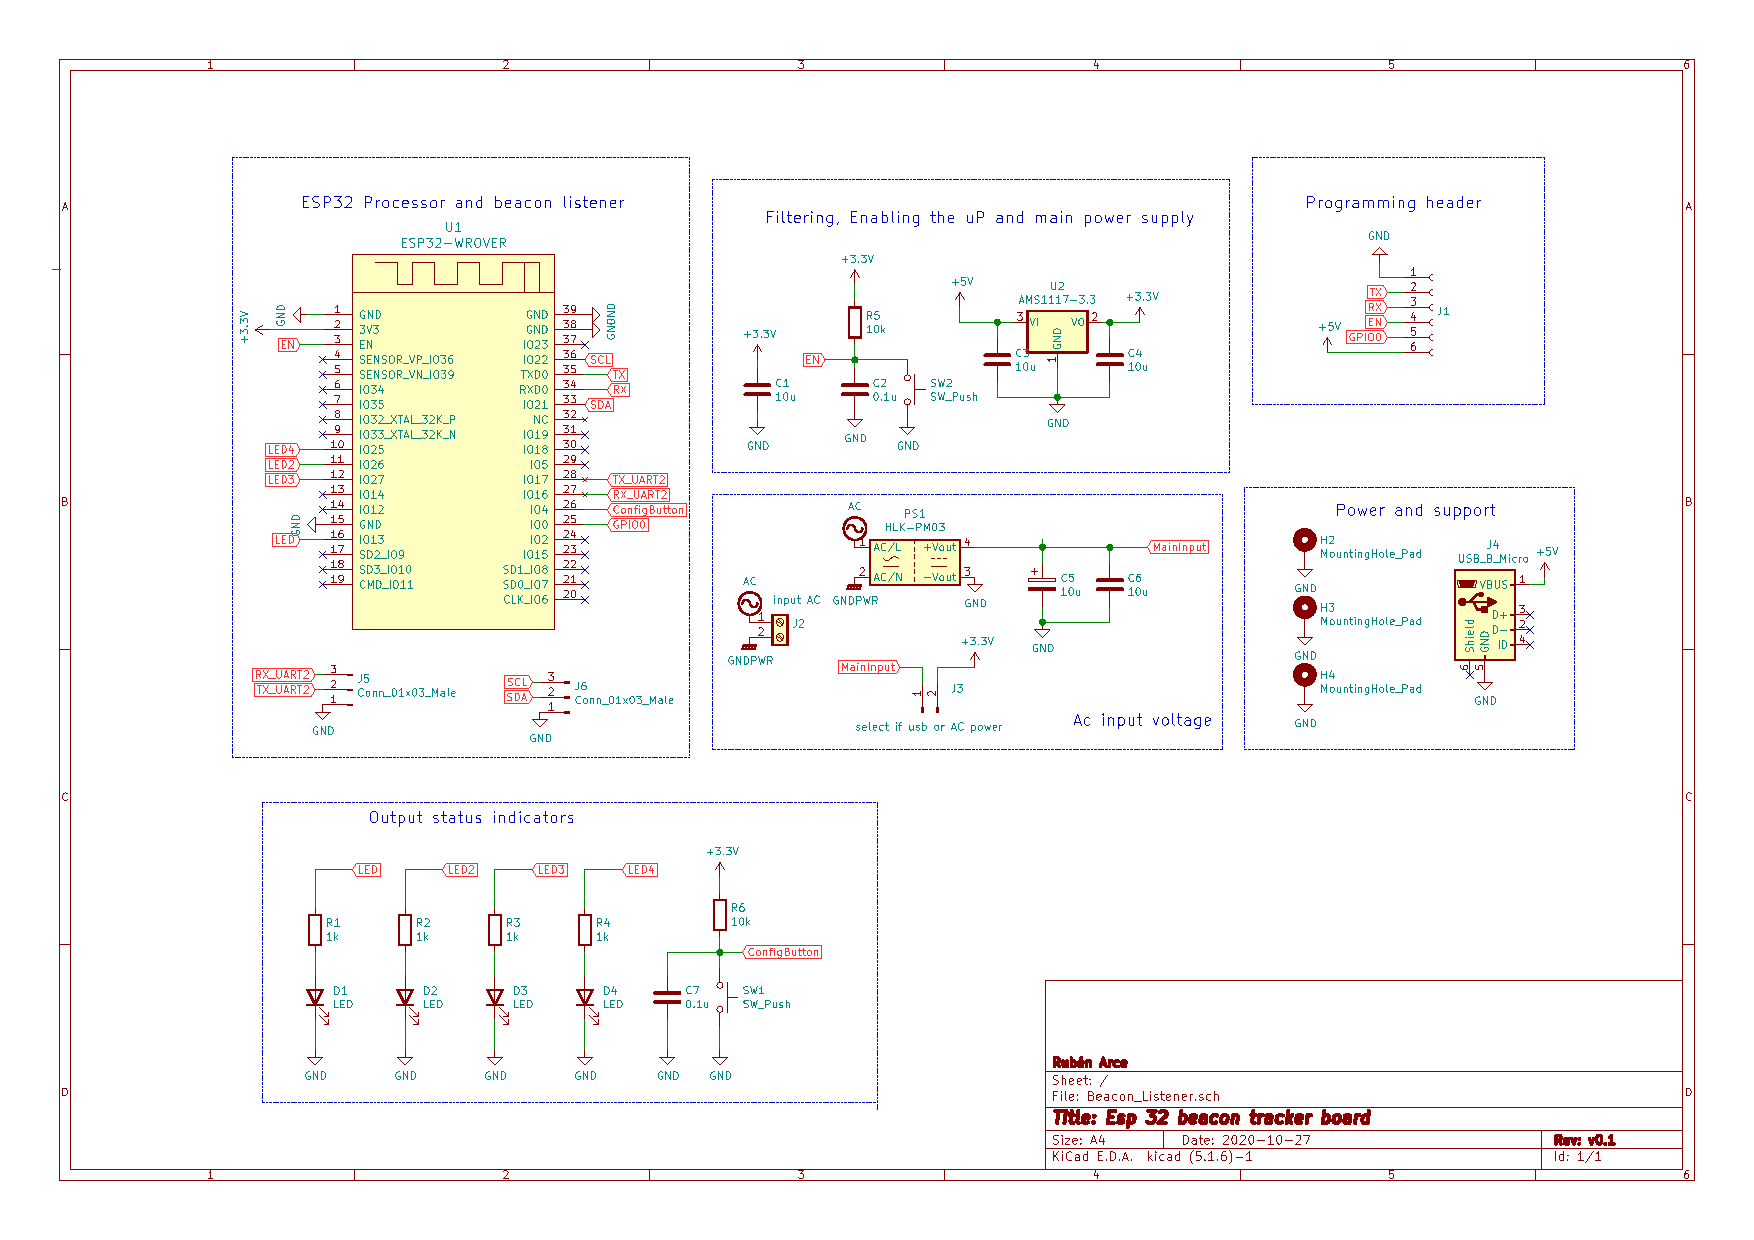
\includepdf[pages=-]{draws_linked.pdf}
\section{Pliego de condiciones}
    \subsection{Prescripciones ténicas generales}
        \subsubsection{Normativa relativa a radiofrecuencia}
            \begin{itemize}
                \item Real Decreto 123/2017: de 24 de febrero, por el que se aprueba el Reglamento
                sobre el uso del dominio público radioeléctrico.
                \item Real Decreto 188/2016: de 6 de mayo, por el que se aprueba el Reglamento 
                por el que se establecen los requisitos para la comercialización, puesta en servicio 
                y uso de equipos radioeléctricos, y se regula el procedimiento para la evaluación de
                la conformidad, la vigilancia del mercado y el régimen sancionador de los equipos de
                telecomunicación.
                \item Orden IET/614/2015: de 6 de abril, por la que se modifica la Orden IET/787/2013,
                de 25 de abril, por la que se aprueba el cuadro nacional de atribución de frecuencias.
                \item Esto viene recogido en la orden ERC/DEC/(01)07.
                \item Ley 9/2014: de 9 de mayo, General de Telecomunicaciones.
                \item Orden CTE/23/2002: de 11 de enero, por la que se establecen condiciones para la presentación de determinados
                estudios y certificaciones por operadores de servicios de radiocomunicaciones. 
            \end{itemize}
        \subsubsection{Normativa relativa a bluetooth y wifi}
            Se ha de tener en cuenta que para poder emplear dispositivos bluetooth se ha de respetar los estándares
            \begin{itemize}
                \item IEEE 802.15.1 define Bluetooth 1.x, que puede alcanzar velocidades de 1 Mbps;
                \item IEEE 802.15.2 recomienda prácticas para utilizar la banda de frecuencia de 2.4 GHz (en convivencia con el wifi)
                \item IEEE 802.15.3 ofrece velocidades de banda ancha (20 Mbps) con Bluetooth;
                \item IEEE 802.15.4 es un estándar que define el nivel físico y el de control de acceso al medio 
                para redes de área personal con tasas bajas de datos (low-rate wireless personal area network, LR-WPAN).
            \end{itemize}
            La clase del disposivo que queda recogida en la siguiente tabla es también un dato a tener en cuenta puesto que no 
            se les aplica la misma normativa.
            \begin{center}
                \addcontentsline{lot}{table}{Potencia y alcance BLE.}
                \begin{tabular}{||c | c |c ||} 
                \hline
                Clase & Potencia  & Alcance aproximado\\ [0.5ex] 
                \hline\hline
                Clase 1 & 100 mW / 20 dBm & 100 m \\ 
                Clase 2 & 2,5 mW / 4 dBm & 5 - 10 m \\ 
                Clase 3 & 1 mW / 0 dBm & 1 m \\ 
                Clase 4 & 0,5 mW / -3 dBm & 0,5 m \\ 
                \hline
                \end{tabular}
            \end{center}
            En nuestro caso y teniendo en cuenta la aplicación, se ha optado por emitir por debajo de los 20 dBm de tal forma
            que no se aplica apenas normativa, debido a que la potencia isotrópica radiada equivalente total será
            inferior a 100 mW.
\section{Presupuestos}
    \subsection{Precios unitarios}
        La tabla de precios se va a elaborar en distintas unidades que corresponden al precio por separado de cada
        una de las PCBs que se han diseñado.
    \subsection{Presupuestos parciales}
            \subsubsection{Placa de circuito impreso emisor Beacon}
                \begin{center}
                    \addcontentsline{lot}{table}{Tabla de precios Emisor Beacon.}
                    \begin{tabular}{||c | c |c ||} 
                    \hline
                    Componente & Cantidad & Precio unitario  \\ [0.5ex] 
                    \hline
                    Resistencia metálica SMD 0805 1k 10  	&1&	 0,009 € \\ 
                    Resistencia metálica SMD 0805 10k 10 	&1&	 0,009 € \\ 
                    Condensador cerámico SMD 0805 0,1uF  	&1&	 0,005 € \\ 
                    Condensador cerámico SMD 0805 10uF   	&1&	 0,016 € \\ 
                    Regulador tensión LDO AMS1117-3.3V   	&1&	 0,098 € \\ 
                    Microcontrolador ESP32-WROOM-32D     	&1&	 2,840 € \\ 
                    Led SMD 0805 verde                   	&1&	 0,013 € \\ 
                    Led SMD 0805 rojo                    	&1&	 0,013 € \\ 
                    Led SMD 0805 naranja                 	&1&	 0,015 € \\ 
                    Batería Litio Ion                    	&1&	 1,520 € \\ 
                    \hline
                    TOTAL                    	            &1&	 4,009 € \\ 
                \hline
                    \end{tabular}
                \end{center}
            \subsubsection{Placa de circuito impreso receptor o gateway}
                \begin{center}
                    \addcontentsline{lot}{table}{Tabla de precios receptor o gateway.}
                    \begin{tabular}{||c | c |c ||} 
                    \hline
                    Componente & Cantidad & Precio unitario  \\ [0.5ex] 
                    \hline
                    Resistencia metálica SMD 0805 1k 10  	&1&	 0,009 € \\ 
                    Resistencia metálica SMD 0805 10k 10 	&1&	 0,009 € \\ 
                    Condensador cerámico SMD 0805 0,1uF  	&1&	 0,005 € \\ 
                    Condensador cerámico SMD 0805 10uF   	&1&	 0,016 € \\ 
                    Regulador tensión LDO AMS1117-3.3V   	&1&	 0,098 € \\ 
                    Microcontrolador ESP32-WROOM-32D     	&1&	 2,840 € \\ 
                    Led SMD 0805 verde                   	&1&	 0,013 € \\ 
                    Led SMD 0805 rojo                    	&1&	 0,013 € \\ 
                    Led SMD 0805 naranja                 	&1&	 0,015 € \\ 
                    Pinheader conector para programación 	&1&	 0,113 € \\ 
                    UART-TTL herramienta de dasarrollo   	&1&	 1,540 € \\ 
                    Power Module AC-DC HI-LINK 3.3V	        &1&	 2,830 € \\ 
                    Screw terminal P=5.08mm	                &1&	 0,097 € \\ 
                    USB Mini B Female                    	&1&	 0,108 € \\ 
                    JST Connector P=2mm                  	&1&	 0,039 € \\ 
                    Jumper connector	                    &1&	 0,017 € \\ 
                    \hline
                    TOTAL                    	            &&	 7,763 € \\ 
                    \hline
                    \end{tabular}
                \end{center}
            \subsubsection{Desarrollo e instalación}
            \begin{center}
                \addcontentsline{lot}{table}{Tabla de precios desarrollo e instalación.}
                \begin{tabular}{||c | c |c ||} 
                \hline
                Componente & Cantidad  & Precio unitario  \\ [0.5ex] 
                 & (h) & € \\ [0.5ex] 
                \hline\hline
                    Diseñador hardware placas circuito impreso   & 10  & 50 \\ 
                    Desarrollador  software sistema embebido     & 350 & 40 \\ 
                    Programador full stack web developer         & 100 & 50 \\ 
                \hline
                \end{tabular}
            \end{center}
    \subsection{Presupuestos total}
        El presupuesto total se compone de la suma de los presupuestos parciales:
        \begin{center}
            \addcontentsline{lot}{table}{Presupuesto general.}
            \begin{tabular}{||c | c |c ||} 
            \hline
            Unidad & Cantidad & Precio  \\ [0.5ex] 
            \hline\hline
            Placa de circuito impreso Beacon o emisor & 10 & 40 \\ 
            Placa de circuito impreso receptor o gateway & 4 & 50 \\ 
            Desarrollo e instalación & 1 & 35 \\ 
            \hline
            \hline
            Total &  & 635€ \\ 
             & IVA 21\%& 133,35 € \\ 
             & & 768,35€ \\ 
            \hline
            \end{tabular}
        \end{center}
        Por lo tanto el presupuesto total con iva asciende a la cantidad de 1234123 4123 y veintimeil euros.
    \subsection{Factores económicos y financieros}
        Para llevar a cabo el estudio de viabilidad económica se ha confeccionado la siguiente tabla donde
        podemos ver los flujos de caja así como la inversión inicial del proyecto:
        \begin{center}
            \addcontentsline{lot}{table}{Flujos de caja de la inversión, VAN y TIR.}
            \begin{tabular}{||c | c |c |c |c ||} 
            \hline
             - & Periodo 0 & Periodo 1& Periodo 2 & Periodo 3  \\ [0.5ex] 
            \hline
            \hline
                Inversión/gastos &1.200,00 € 	& 4.523,60 € 	& 4.523,60 € 	& 4.523,60 € \\ 
                Flujos de caja  &-1.200,00 € 	& 1.776,40 € 	& 3.476,40 € 	& 476,40 €   \\ 
            \hline
            \end{tabular}
        \end{center}
        Se ha de tener en cuenta que esto es un proyecto real y que los gastos son verídicos y surgen del pago de
        las cuotas de autónomos, electricidad y gasolina que supone trabajar desde casa. Con todo esto y fijando una cuota
        de COK o coste de oportunidad de capital o mínima rentabilidad admisible para afrontar la realización del
        proyecto, se ha establecido de un 3\%.
    \subsubsection{TIR y VAN}
        El análisis de la tasa de interés de retorno y del valor actual neto son los que se recogen en la siguiente tabla:
        \begin{center}
            \addcontentsline{lot}{table}{Flujos de caja de la inversión, VAN y TIR.}
            \begin{tabular}{||c | c ||} 
            \hline
                TIR &4.237,47 € \\ [0.5ex] 
                VAN & 164 \% \\ [0.5ex] 
            \hline
            \end{tabular}
        \end{center}
        Teniendo en consideración todos los aspectos menciones, se puede concluir que la inversión es rentable y asumible
        si se presupone una venta anual de proyectos con diferentes características.
        Es importante mencionar que este escenario no es real al 100\% debido a que no solo se venderá este producto, igualmente al ser 
        ventas puntuales no se requiere un posterior tratamiento con el cliente y esto hace que sea más rentable.
\section{Bibliografía}
    \begin{itemize}
        \item Accent systems. (s.f.). accent systems. https://accent-systems.com/es/producto/ibks-105/ 
        \item Apple. (2014). Getting Started with iBeacon [version 1.0].
        \item Bluetooth. (s.f.). Blueetooth. https://www.bluetooth.com/ 
        \item Cejas, A. y Chardon, A. (2019). Algoritmos avanzados de posicionamiento en interiores
        \item Chruszczyk, L. y Zajac, A. (2016). Comparison of Indoor/Outdoor, RSSI-Based Positioning Using 433, 868 or 2400 MHz ISM Bands. Intl Journal of Electronics and Telecommunications, 32(4), 395-399.
        \item ESP-IDF Release V4.2. (2020, 7 de diciembre). Expressif loT Development Framework. Espressif. https://github.com/espressif/esp-idf 
        \item Espressif Systems. (2020). ESP32 Hardware Design Guidelines [version 3.0].
        \item Espressif Systems. (2020). ESP32 Technical Reference Manual [version 4.3].
        \item Jayakody, J. A., Lokuliyana, S., Chathurangi, D. y Vithana, D. (2016). Indoor Positioning:
         Novel Approach for Bluetooth Networks using RSSI Smoothing. International Journl of Computer Applicatios, 137(13), 26-32.
        \item Jefatura del Estado. (2014, 5 de mayo). Ley 114. Por la que se expide la Ley General de
        Telecomunicaciones. BOE-A-2014-4950. https://www.boe.es/buscar/act.php?id=BOE-A-2014-4950 
        \item Ministerio de Ciencia y Tecnología de España. (2002, 11 de enero). Orden CTE/23/2002. Por la que se establecen condiciones para la presentación de determinados estudios y certificaciones por
        operadores de servicios de radiocomunicaciones.  \href{https://www.boe.es/diario_boe/txt.php?id=BOE-A-2002-694}{BOE-A-2002-694.}
        \item Nordic Semiconductor. (2017). nRF52832 Product Specification v1.4.
        \item Pattnayak, T. y Thanikachalam, G. (2018). Antenna Design and RF Layout Guidelines [application notes]. Cypress. http://www.cypress.com/go/AN91445 
        \item Shang, F., Su, W., Wang, Q., Gao, H. y Fu, Q. (2014). A Location Estimation Algorithm Based on RSSI Vector Similarity Degree. International Journal of Distributed Sensor Networks. http://dx.doi.org/10.1155/2014/371350 
        \item ShareLaTeX. (s.f.). ShareLaTeX. https://www.sharelatex.com/ 
        \item Shezhen Radioland Technology. Bluetooth Smart Module BLE4.0 NRF51822-Beacon Datasheet.
        \item Tabibi, M. A. y Shahnewaz, A. (2012). RSSI Based Location [tesis de maestría, Universidad Politécnica de Milán].
        \item utilizando la combinación de distintos tipos de sensores [trabajo de fin de grado, Universidad Nacional del Centro de la Provincia de Buenos Aires].
        \item Vara, N., Poletto, G.A., Cáceres, M. y Busso, A. J. (2015). Cálculo de distancia entre los nodos de una red inalámbrica Zigbee en función del parámetro RSSI. Extensionismo, innovación y trasferencia tecnológica. Claves para el desarrollo, 2, 8-13.
        \item Yu, X. (2014). Diseño de antenas de tipo parche para un transceptor WiMAX basado en el chip MAX2838 [trabajo fin de grado, Escuela Politécnica Superior de la Universidad Autónoma de Madrid].
    \end{itemize}
\end{document} 